\documentclass[reqno]{amsart}

\usepackage[margin=2.5cm]{geometry}
\usepackage[pdftex]{graphicx}
\usepackage[utf8]{inputenc}
\usepackage[T1]{fontenc}
\usepackage{textcomp}
\usepackage{babel}
\usepackage{amsmath, amssymb, amsthm, amscd}
\usepackage[colorlinks=true,linkcolor=blue]{hyperref}
\usepackage{float}
\usepackage{mathrsfs}
%\usepackage{enumitem}
%% for identity function 1:
\usepackage{bbm}
%%For category theory diagrams:
\usepackage{tikz-cd}
%%For code (e.g. python) in latex:
%\usepackage{listings}
%
%Usage: 
%\begin{lstlisting}[language=Python]
%\end{lstlisting}

\newcommand{\incfig}[2][1]{%
\def\svgwidth{#1\columnwidth}
\import{./figures/}{#2.pdf_tex}
}


\theoremstyle{plain}% default
\newtheorem{theorem}{Theorem}[section]
\newtheorem{lemma}[theorem]{Lemma}
\newtheorem{proposition}[theorem]{Proposition}
\newtheorem{corollary}[theorem]{Corollary}


\theoremstyle{definition}
\newtheorem{definition}[theorem]{Definition}
\newtheorem{example}[theorem]{Example}
\newtheorem{exercise}[theorem]{Exercise}


\theoremstyle{remark}
\newtheorem*{remark}{Remark}
\newtheorem*{note}{Note}
\newtheorem*{solution}{Solution}






% figure support
\usepackage{import}
\usepackage{xifthen}
\pdfminorversion=7
\usepackage{pdfpages}
\usepackage{transparent}

\pdfsuppresswarningpagegroup=1

\setlength\parindent{0pt}

\newcommand{\qedwhite}{\hfill \ensuremath{\Box}}

%Inequalities
\newcommand{\cycsum}{\sum_{\mathrm{cyc}}}
\newcommand{\symsum}{\sum_{\mathrm{sym}}}
\newcommand{\cycprod}{\prod_{\mathrm{cyc}}}
\newcommand{\symprod}{\prod_{\mathrm{sym}}}

%Linear Algebra

\DeclareMathOperator{\Span}{span}
\DeclareMathOperator{\Ima}{Im}
\DeclareMathOperator{\diag}{diag}
\DeclareMathOperator{\Ker}{Ker}
\DeclareMathOperator{\ob}{ob}
\DeclareMathOperator{\sk}{sk}
\DeclareMathOperator{\Vect}{Vect}
\DeclareMathOperator{\Set}{Set}
\DeclareMathOperator{\Group}{Group}
\DeclareMathOperator{\Ring}{Ring}
\DeclareMathOperator{\Ab}{Ab}
\DeclareMathOperator{\Top}{Top}
\DeclareMathOperator{\hTop}{hTop}
\DeclareMathOperator{\Htpy}{Htpy}
\DeclareMathOperator{\Cat}{Cat}
\DeclareMathOperator{\CAT}{CAT}
\DeclareMathOperator{\Cone}{Cone}
\DeclareMathOperator{\dom}{dom}
\DeclareMathOperator{\cod}{cod}
\DeclareMathOperator{\Aut}{Aut}
\DeclareMathOperator{\Mat}{Mat}
\DeclareMathOperator{\Fin}{Fin}
\DeclareMathOperator{\rel}{rel}
\DeclareMathOperator{\Int}{Int}
\newcommand{\SL}{{\mathrm{SL}}}
\newcommand{\mobgp}{{\mathrm{PSL}_2(\mathbb{C})}}
\newcommand{\Hom}{{\mathrm{Hom}}}
\newcommand{\id}{{\mathrm{id}}}
\newcommand{\Mod}{{\mathrm{Mod}}}
\newcommand{\ud}{{\mathrm{d}}}
\newcommand{\Vol}{{\mathrm{Vol}}}
\newcommand{\Area}{{\mathrm{Area}}}
\newcommand{\diam}{{\mathrm{diam}}}

\newcommand{\reg}{{\mathtt{reg}}}
\newcommand{\geo}{{\mathtt{geo}}}

\newcommand{\tori}{{\mathcal{T}}}
\newcommand{\cpn}{{\mathtt{c}}}
\newcommand{\pat}{{\mathtt{p}}}


%Row operations
\newcommand{\elem}[1]{% elementary operations
\xrightarrow{\substack{#1}}%
}

\newcommand{\lelem}[1]{% elementary operations (left alignment)
\xrightarrow{\begin{subarray}{l}#1\end{subarray}}%
}

%SS
\DeclareMathOperator{\supp}{supp}
\DeclareMathOperator{\Var}{Var}

%NT
\DeclareMathOperator{\ord}{ord}

%Alg
\DeclareMathOperator{\Rad}{Rad}
\DeclareMathOperator{\Jac}{Jac}

\DeclareMathAlphabet{\pazocal}{OMS}{zplm}{m}{n}
\newcommand{\unif}{\pazocal{U}}

\title{Curves and Surfaces - Schlichtkrull}
\date{}


\begin{document}
\maketitle
\section{Parametrized curves and surfaces and trace}
    \begin{definition}[parametrized continuous curve]
        A \textbf{parametrized continuous curve} in $\mathbb{R}^{n}$ is
        a continuous map $\gamma  \colon I \to \mathbb{R}^{n}$, for $n\ge 2$, where
        $I \subset \mathbb{R}$ is an open interval.\\
        The image set $\mathcal{C} = \gamma (I) \subset \mathbb{R}^{n}$ si
        called the \textbf{trace} of the curve.\\
        A point in the trace, which corresponds to more than one parameter value
        $t$, is called a \textbf{self-intersection} of the curve.
    \end{definition}
    \begin{example}{circle}
        The curve $\gamma  \colon \mathbb{R} \to \mathbb{R}^2$ given by
        $t\mapsto \left( r \cos t, r \sin t \right) $ parametrizes a curve and
        all points in the trace are self-intersections because values 
        $t+ 2 \pi k$ correspond to the same point for all $k \in \mathbb{Z}$.
    \end{example}
    \begin{definition}[smooth curve]
        A parametrized continuous curve for which the map
        $\gamma  \colon I \to \mathbb{R}^{n}$ is differentiable up to all
        orders is called a parametrized smooth curve; i.e., if each of the
        component functions of $\gamma$ are infinitely differentiable.
    \end{definition}
    \begin{note}
        In these notes, we will only be concerned with smooth curves, and
        therefore we adopt the convention that from now on a parametrized curve
        is smooth, unless otherwise mentioned.
    \end{note}
    \begin{example}{Ellipse}
        A map $\gamma (t) = \left( a \cos t, b \sin t \right) $, where 
        $a,b > 0$ are constants, parametrizes the \textbf{ellipse}
        $\mathcal{C} = \left\{ \left( x,y \right)  \mid 
        \frac{x^2}{a^2} + \frac{y^2}{b^2} = 1\right\} $.
    \end{example}
\begin{example}[hyperbola]
    Let $\gamma (t) = \left( a \cosh t , b \sinh t \right) $ where $a,b >0$ and
    \[
    \cosh t = \frac{e^{t} + e^{-t}}{2}, \quad \sinh t = \frac{e^{t}-e^{-t}}{2}.
    \] 
    Then
    \[
    \mathcal{C = \left\{ \left( x,y \right)  \mid 
    \frac{x^2}{a^2} - \frac{y^2}{b^2} = 1 , x >0 \right\} }.
    \] 
    \begin{figure}[H]
        \centering
        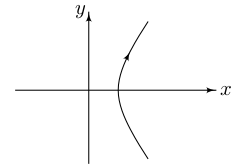
\includegraphics[width=0.3\textwidth]{hyperbola.png}
        \label{fig:hyperbola-png}
    \end{figure}
\end{example}
\begin{example}[Helix]
    The space curve $\gamma(t) = \left( \lambda t, r \cos \left( \omega
    t \right) , r \sin \left( \omega t \right)  \right) $ where
    $r >0$ and $\lambda, \omega \neq 0$ are constants, is called
    a \textbf{helix}.
    \begin{figure}[H]
        \centering
        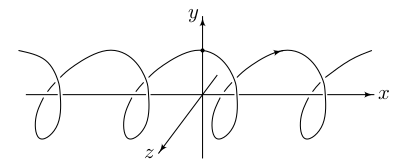
\includegraphics[width=0.5\textwidth]{helix.png}
        \label{fig:helix-png}
    \end{figure}
\end{example}
\subsection{Surfaces}
\begin{definition}[Continuous surface]
    A \textbf{parametrized continuous surface} in $\mathbb{R}^3$ is
    a continuous map $\sigma  \colon U \to \mathbb{R}^3$ where
    $U \subset \mathbb{R}^2$ is an open, non-empty set.
    \begin{figure}[H]
        \centering
        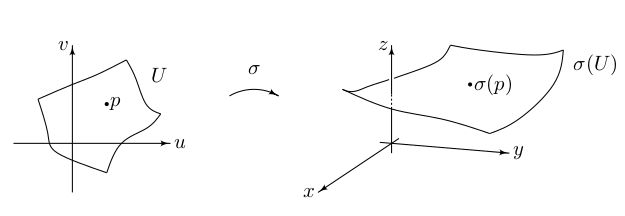
\includegraphics[width=0.5\textwidth]{surface.png}
        \label{fig:surface-png}
    \end{figure}
\end{definition}
\begin{definition}[Smooth maps]
    If $U$ and  $V$ are open subsets of $\mathbb{R}^{n}$ 
    and $\mathbb{R}^{m}$, respectively, a function
    $F  \colon U \to V$ is said to be \textbf{smooth}
    (or  \textbf{$C^{\infty}$}, or \textbf{infinitely differentiable}) if each
    of its component functions has continuous partial derivatives of all
    orders.
\end{definition}
\begin{note}
    We adopt the convention that a \textit{parametrized surface is smooth,
    unless otherwise mentioned}.
\end{note}
\begin{example}[Plane]
    Let $p, q_1, q_2 \in \mathbb{R}^3$ be fixed vectors and let
    \[
    \sigma \left( u,v \right) = p + uq_1 + vq_2
    \] 
    for $\left( u,v \right) \in U = \mathbb{R}^2$. Then
    $\sigma$ is a parametrized surface. If $q_1, q_2$ are linearly independent,
    the image $\sigma(U)$ is a plane. Otherwise, it is a line or a point.
\end{example}
\begin{example}[Sphere]
    Let
    \[
    \sigma (u,v) = \left( \cos u \cos v, \cos u \sin v, \sin u \right) 
    \] 
    where $\left( u,v \right) \in \mathbb{R}^2$. This is the standard
    parametrization of the unit sphere
    \[
    S^2 = \left\{ \left( x,y,z \right) \in \mathbb{R}^3  \mid 
    x^2 + y^2 + z^2 = 1 \right\} .
    \] 
    The parameters $u$ and $v$ are called \textit{latitude} and
    \textit{longitude}, and together they are called \textbf{spherical
    coordinates}.
    \begin{figure}[H]
        \centering
        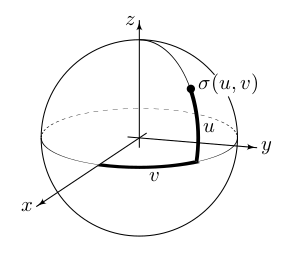
\includegraphics[width=0.3\textwidth]{spherical-coordinates.png}
        \label{fig:spherical-coordinates-png}
    \end{figure}
    This parametrization covers the total sphere, but it is not injective. On
    the other hand, if say $u \in \left( -\frac{\pi}{2},\frac{\pi}{2} \right)
    $ and $v \in \left( -\pi, \pi \right) $, then $\sigma$ is injective, but it
    is not surjective since a half-circle on the back of the sphere is not in
    the image.
\end{example}
\begin{example}[Cone]
    Let $\lambda  > 0$ and
    \[
    \sigma \left( u,v \right) = \left( \lambda  u \cos v,
    \lambda  u \sin v , u\right) 
    \] 
    where $\left( u,v  \right) \in \mathbb{R}^2$. This gives the cone
    $\left\{ \left( x,y,z \right)  \mid x^2 + y^2 = \lambda^2 z^2 \right\} $
\end{example}
\subsection{Graphs}
\begin{example}[Graph of affine linear maps]
    Graph of $h(t) = at+b, \mathbb{R} \to \mathbb{R}, a,b \in \mathbb{R}$ is
    the line in $\mathbb{R}^2$ parametrized by $(t, at+b)$.
    All lines not perpendicular to the $x$-axis can be parametrized in this
    fashion.\\
    Similarly, the graph of an affine linear map $h(t) = at+b, \mathbb{R}
    \to \mathbb{R}^2$ where $a,b \in \mathbb{R}^2$ is the line in
    $\mathbb{R}^3$ parametrized by
    $\left( t, a_1t+b_1, a_2t+b_2 \right) $. All lines of direction not
    perpendicular to the $x$-axis can be parametrized in this fashion.
\end{example}
\begin{example}[Surfaces that are graphs]
    If $h  \colon U \to \mathbb{R}$ is a smooth map defined on
    $U \subset \mathbb{R}^2$, then its graph is a surface
     \[
    \left\{ \left( u,v, h(u,v) \right)  \mid 
    (u,v) \in U \right\} \subset \mathbb{R}^3.
    \] 
    Equipped with the map
    \[
    \sigma (u,v) = \left( u,v,h(u,v) \right) , \quad (u,v) \in U,
    \] 
    the graph is clearly a parametrized smooth surface.
\end{example}
\begin{example}[Planes not perp to $xy$-plane]
    The graph of an affine linear function $\mathbb{R}^2 \to \mathbb{R}$ is
    a plane in $\mathbb{R}^3$. Say $h(u,v) = au+bv +c$ where
    $a,b,c \in \mathbb{R}$, then $\sigma  (u,v) = \left( u,v,
    au + bv + c\right) $. All planes, except those which are perpendicular to
    the $xy$-plane, can be parametrized in this fashion.
\end{example}
\begin{example}[Hemisphere]
    The graph of the map $h(u,v) = \sqrt{1 - u^2 - v^2} $, defined on
    $B(0,1) = \left\{ 
    \left( u,v \right) \in \mathbb{R}^2  \mid 
u^2 + v^2 < 1 \right\} $ is a hemisphere.
\end{example}
\subsection{Level sets}
A plane curve is often described by means of an equation: e.g. a line
represented by $ax+by =c, a,b,c \in \mathbb{R}$ and $(a,b) \neq (0,0)$.\\
Similarly, a surface can be described by an equation. For example, a plane in
$\mathbb{R}^3$ is the set of solutions to an equation
$ax +by +cz = d$ where $\left( a,b,c \right) \neq 
\left( 0,0,0 \right) $.
\begin{definition}[Level sets]
    Let $\Omega \subset \mathbb{R}^{n}$ be open and let 
    $f  \colon \Omega \to \mathbb{R}$ be continuous. The \textbf{level sets}
    for
    $f$ are the sets
    \[
    \mathcal{C} = \left\{ x \in \Omega  \mid  f(x) = c \right\} 
    \] 
    of solutions in $\Omega$ to the equation $f(x) = c$, where
    $c \in \mathbb{R}$ is fixed.
\end{definition}
\begin{definition}[Critical points]
    Let $f  \colon \Omega \to \mathbb{R}$ be smooth, where $\Omega \subset
    \mathbb{R}^{n}$ is open. A point $p \in \Omega$ is called \textbf{critical}
    if
    \[
        \frac{\partial f}{\partial x_1}(p) = \ldots = 
        \frac{\partial f}{\partial x_n}(p) = 0.
    \] 
\end{definition}

\begin{example}[]
    The solutions to $ax + by = c$ comprise levels sets for
    $f(x,y)=ax+by$. If $(a,b) \neq (0,0)$ then there are no critical points. In
    this case, the set of solutions form a line, hence can be parametrized as
    a curve. If $(a,b) = (0,0)$, then $f$ is the trivial function and all
    points are critical.
\end{example}
\begin{example}[]
    Consider $f(x,y) = xy = 0$. Here
    $\frac{\partial f}{\partial x} = y$ and
    $\frac{\partial f}{\partial y}=x$, and hence the origin is the only
    critical point. In fact, the level set given by $f(x,y)=0$ is the union of
    two axes, which exactly fails to be a 'reasonable' curve at the origin.
\end{example}

\subsection{The implicit function theorem for two variables}
The implicit function theorem describes conditions under which a given equation
in two variables can be solved to obtain one of the variables as a function of
the other variables.

\begin{theorem}[Implicit function theorem for two
    variables]\label{implicit-function-two-var}
    Let $f  \colon \Omega \to \mathbb{R}$ be a smooth function where
    $\Omega \subset \mathbb{R}^2$ is open. Let
    \[
    \mathcal{C} = \left\{ \left( x,y \right) \in \Omega
     \mid  f(x,y) = c \right\} 
    \] 
    be the set of solutions to the equation
    $f(x,y) = c$. Let $p = \left( x_0,y_0 \right) 
    \in \mathcal{C}$ be given, and assume that
    $\frac{\partial f}{\partial y}\neq 0$ at $p$.\\
    Then there exist open intervals $I$ and $J$ around $x_0$ and $y_0$,
    respectively, such that $I \times J \subset \Omega$ and
    there exists a smooth map $h  \colon I \to J$ such that
    \[
    \mathcal{C} \cap I \times J = \left\{ \left( x, h(x) \right)  \mid x \in I \right\}
    ,\label{eq:implicit-function-theorem}\tag{$\omega$}
    \] 
    that is, in the neighborhood $I \times J$ of $p$, $\mathcal{C}$ is the graph of $h$.
\end{theorem}

\begin{figure}[H]
    \centering
    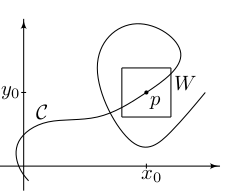
\includegraphics[width=0.3\textwidth]{implicit-function-thm-two}
    \label{fig:implicit-function-thm-two}
\end{figure}

\begin{proof}
    Assume for simplicity that $c=0$ and $\frac{\partial f}{\partial x} > 0$ at
    $p$. These properties can be arranged by a simple replacement of
    $f$ which does not affect the set $\mathcal{C}$.
    By continuity of $\frac{\partial f}{\partial y}$ and openness of $\Omega$,
    we can choose $\delta > 0$ such that
    $\left[ x_0- \delta, x_0 + \delta \right] \times \left[ 
    y_0 - \delta, y_0 + \delta \right] \subset \Omega $ and such that
    $\frac{\partial f}{\partial y} > a$  for some $a > 0$ on this neighborhood.
    Then $y \mapsto f(x,y)$ is strictly increasing on 
    $\left[ y_0 - \delta, y_0 + \delta \right] $ for each fixed
    $x$ with $\left| x-x_0 \right| < \delta$.\\
    In particular, since $p \in \mathcal{C}$, we have
    $f(p) = f\left( x_0, y_0 \right) =0$ and hence
    \[
    f\left( x_0, y_0 - \delta \right) <0 \quad \text{and} \quad
    f\left( x_0, y_0 + \delta \right) >0.
    \] 
    By continuity in $x_0$ of each of the maps $x \mapsto f(x, y_0 \pm
    \delta)$, there exists a positive number $\eta \le \delta$ such that
    $f\left( x, y_0- \delta \right) <0$ and
    $f\left( x, y_0+ \delta \right) >0$ for all $x$ with
    $\left| x - x_0 \right|  < \eta$.\\
    Let $I = \left( x_0 - \eta, x_0 + \eta \right) $ and let
    $x \in I$. We wish to define a map $h  \colon I \to J$.\\
    
    Since $y \mapsto f(x,y)$ is strictly increasing and continuous
    and $f\left( x, y_0- \delta \right) < 0$ and
    $f\left( x, y_0+ \delta \right) \ge $, there exists a unique $y$ between
    $y_0 - \delta$ and $y_0 + \delta$ with $f(x,y) = 0$. This value of
    $y$ is denoted $h(x)$. Then $h$ maps $I$ into $J
    = \left( y_0 - \delta, y_0 + \delta \right) $ and satisfies
    $f\left( x, h(x) \right) =0$.\\
    The identity of the sets in \eqref{eq:implicit-function-theorem}
    follows from the uniqueness of $y$.\\
    \linebreak
    It only remains to show that $h$ is smooth. We first show that
    $h$ is continuous. Fix $x \in I$ and let $y = h(x)$. Then
    $f(x,y)=0$. Choose $\delta_x \in \mathbb{R}$ sufficiently small that
    $x + \delta_x \in I$. Define
    $\delta_y$ such that $y+ \delta_y = h(x+ \delta_x)$, then also
    $f\left( x+\delta_x , y + \delta_y \right) =0$.\\
    The asserted continuity amounts to showing that $\delta_y \to 0$ as
    $\delta_x \to 0$. The map
    \[
    t \mapsto \varphi(t) = f\left( x+ t \delta_x, y + t \delta_y \right) 
    \] 
    is zero both for $t=0$ and $t=1$. By the mean value theorem (Rolle's
    theorem), there exists a number $\theta \in \left( 0,1 \right) $ depending
    on $\delta_x$ such that
    \[
    \varphi' \left( \theta \right) =0.
    \] 
    Differentiating $\varphi$ by means of the chain rule, we thus obtain
    \[
    \frac{\partial f}{\partial x} \left( x+ \theta \delta_x,
    y +  \theta \delta_y \right) \delta_x +
    \frac{\partial f}{\partial y}\left( x+ \theta \delta_x , 
    y+ \theta \delta_y \right) \delta_y = 0
    \] 
    Hence
    \[
    \delta_y = - \frac{\frac{\partial f}{\partial x}\left( x+ \theta \delta_x,
    y + \theta \delta_y \right) }{\frac{\partial f}{\partial y} 
    \left( x + \theta \delta_x , y + \theta \delta_y \right) } \delta_x
    \] 
    and since $\left| \frac{\partial f}{\partial x} \right| $ is bounded, and
    $\frac{\partial f}{\partial y} \ge a >0$, it follows that $\delta_y \to 0$ 
    when $\delta_x \to 0$, as claimed.\\
    Next we prove that $h$ is differentiable, which with the notation from
    above amounts to the convergence of 
    $\frac{\delta_y}{\delta_x}$ as $\delta_x \to 0$. In fact, since
    $\frac{\partial f}{\partial x}$ and $\frac{\partial f}{\partial y}$ are
    continuous, this follows immediately from the equation above.
    Moreover, the limit is given by
    \[
    \lim_{\delta_x \to 0} \frac{\delta_y}{\delta_x}
    = - \frac{\frac{\partial f}{\partial x}(x,y)}{
    \frac{\partial f}{\partial y}(x,y)}.
    \] 
    Hence $h$ is differentiable and satisfies
    \[
    h'(x) = - \frac{\frac{\partial f}{\partial x}(x,h(x))}{
    \frac{\partial f}{\partial y}(x,h(x))}.
    \] 
    Finally, we prove by induction that $h$ is smooth. Assuming that $h$ is $r$ 
    times differentiable for some $r \in \mathbb{Z}_+$, we see from the
    equation above that so is $h'$. Hence $h$ is $r+1$ times differentiable.
\end{proof}
\begin{corollary}[]
    Let $f  \colon \Omega \to \mathbb{R}$ be a smooth function, where
    $\Omega \subset \mathbb{R}^2$ is open. Let
    \[
    \mathcal{C} = \left\{ \left( x,y \right) \in \Omega  \mid 
    f(x,y) = c \right\} 
    \] 
    and let $p = \left( x_0, y_0 \right) \in \mathcal{C}$. Assume that
    $p$ is not a critical point.\\
    Then there exists an open rectangle $W \subset \Omega$ around $p$, such
    that $\mathcal{C} \cap W$ is the graph of a smooth function $h$, considered
    either as $y = h(x)$ or as $x = h(y)$.\\
    In particular, it follows that the level set can be parametrized as
    a smooth curve in a neighborhood of each non-critical point.
\end{corollary}
\begin{proof}
    Either $\frac{\partial f}{\partial y}\neq 0$ or
    $\frac{\partial f}{\partial x}\neq 0$. In the first case,
    $y = h(x)$ by theorem \ref{implicit-function-two-var}. In the other case,
    interchange $x$ and $y$ in the theorem, to get the case
    $x = h(y)$.
 \end{proof}

 \subsection{The implicit function theorem for more variables}



































\end{document}
